%storm
\documentclass[../../main/main.tex]{subfiles}


\begin{document}
\title{Background}


%%%%%%%%%%%%%%%%%%%%% Chapter STORM %%%%%%%%%%%%%%%
\chapter{Background And Introduction to STORM}\label{chp:srorm}
This chapter provides an introduction to \Gls{storm}.  STORM falls within the field of \Gls{se} and the sub-discipline of \Gls{sse}. To familiarize (or refresh) the reader, this chapter begins with some background on \Gls{se} and \Gls{sse}.  The SE concept of system life-cycle phases and the SSE Framework are introduced.  Following this, STORM and it's components (STPA-Sec and CSBD) are introduced.  The chapter concludes with a discussion of the patrol base operations as a sample systems to which STORM is applied.

%%%%%%%%%%%%%%%%%%%%% Section SE %%%%%%%%%%%%%%%
\section{Systems Engineering}\label{sec:stormse}
\begin{quote}
\textit{"Systems Engineering is an interdisciplinary approach and means to enable the realization of successful systems. It focuses on defining customer needs and required functionality early in the development cycle, documenting requirements, then proceeding with design synthesis and system validation while considering the complete problem..."
}\end{quote}
International Council on Systems Engineering 

A system is a set of interacting and interdependent components that act as a whole,  through various mechanisms, to perform some function. Systems engineering is a multidisciplinary approach to solving problems related to large and complex man-made systems.  It focuses on stakeholder needs and assets while minimizing asset losses.  It focuses on building the right product.  It avoids building the wrong product or building the right product incorrectly.  

According to Holstein and Bode's, who summarized systems engineering for the Encyclopedia Britannica, systems engineering probably developed from the overlapping of engineering concepts from different fields. They note that, for example, both chemical and mechanical engineering focus on heat transfer, and cybernetics and computer theory are both subdisciplines of electrical and electronics engineering.   But, at its core is the scientific methodology and the use of mathematical modeling.  Holstein and Bode link the more recent emergence of systems engineering to the communications industry (telephony, in particular) and Britain's post-World War II operations research.

The emergence of systems engineering and its growing popularity is linked to the growing complexity of systems.  Systems are composed more and more of numerous interacting parts.  These interacting parts often exhibit emergent properties.  These are properties that arise from the interactions of many components.  These properties are not attributable to any one component and thus require a systems-thinking perspective. Holstein and Bode site the Nike Ajax U.S. Air Defense System as one of the earlier examples of these system-level emergent properties. Tactical range of the Ajax requires consideration of multiple factors including aerodynamic design, maneuverability provided by the control systems, warhead size and weight, etc.  Other factors include feedback from radar and the autopilot.  Achieving tactical range emerges from analysis of the many interacting components.  

Systems engineering is often employed in the communications and computing industries. But, it works in any field that works with large complex systems.  The applicability of systems engineering to other fields is promoted, in part, by the increased capacity to manage complex systems that arise from the increased computational power available.  Systems engineering is a growing field and demands for systems engineers will continue to grow as systems become more and more complex.

The relevant authoritative \gls{se} standards are defined in ISO/IEC/IEEE 24748-1 \cite{}and ISO/IEC/IEEE 25288\footnore{These standards reference other relevant standards.}.  These standards define the concept of system life-cycle phases: concept, development, production, utilization, support, and retirement.  The concept and development phases are the focus of \gls{storm} because safety and security should be considered during the design phase.  However, the support phase is also relevant for re-envisioning and updating the system.  


Authoritative guidelines and standards on systems engineering can be found in ISO/IEC/IEEE 24748-1 and ISO/IEC/IEEE 25288.  These works describe six distinct phases of a system's life cycle: 
%%%%%%%%%%%%%%%%%%%%% Section SSE %%%%%%%%%%%%%%%
\section{Systems Security Engineering}\label{sesc:sse}
\begin{quote}
\textit{"The ultimate objective is to obtain trustworthy secure systems that are fully capable of supporting critical missions and business operations while protecting stakeholder assets, and to do so with a level of assurance that is consistent with the risk tolerance of those stakeholders."}
\end{quote}
Ron Ross (NIST) (Quoted from NIST SP 800-160)

Systems Security Engineering \glsentryshort{sse} is a subdiscipline of Systems Engineering.  It applies scientific, mathematical, and related technical concepts and procedures to engineer trustworthy systems that meet stakeholder needs. 

Systems Security Engineering probably developed alongside systems engineering.  But, the need for security in all systems is becoming more and more evident in today's technology-dependent society.  In the authoritative document on SSE (National institute for Standardization and Technology (NIST) Special Publication 800-160 vol 1), the abstract states

"With the continuing frequency, intensity, and adverse consequences of cyber-attacks, disruptions, hazards, and other threats to federal, state, and local governments, the military, businesses, and the critical infrastructure, the need for trustworthy secure systems has never been more important to the long-term economic and national security interests of the United States. Engineering-based solutions are essential to managing the growing complexity, dynamicity, and interconnectedness of today?s systems, as exemplified by cyber-physical systems and systems-of-systems, including the Internet of Things."

Systems Security Engineering is practiced whenever security is a component of systems engineering.  As a subspecialty of systems engineering, SSE focuses on stakeholder assets and loss avoidance or mitigation.  It is a multidisciplinary approach that considers emergent properties which arise from the complexity of large systems.
   

\subsection{Systems Security Engineering Framework}
The authoritative document on SSE is the National Institute of Standardization and Technology (NIST) Special Publication 800-160 Volumes 1 and 2.  In particular, volume 1 defines the SSE Framework.  This framework defines SSE activities that ensure the stakeholder's definition of security and asset valuation is understood.  A diagram of the framework is shown in figure \ref{sseframework}.

\begin{figure}[h]
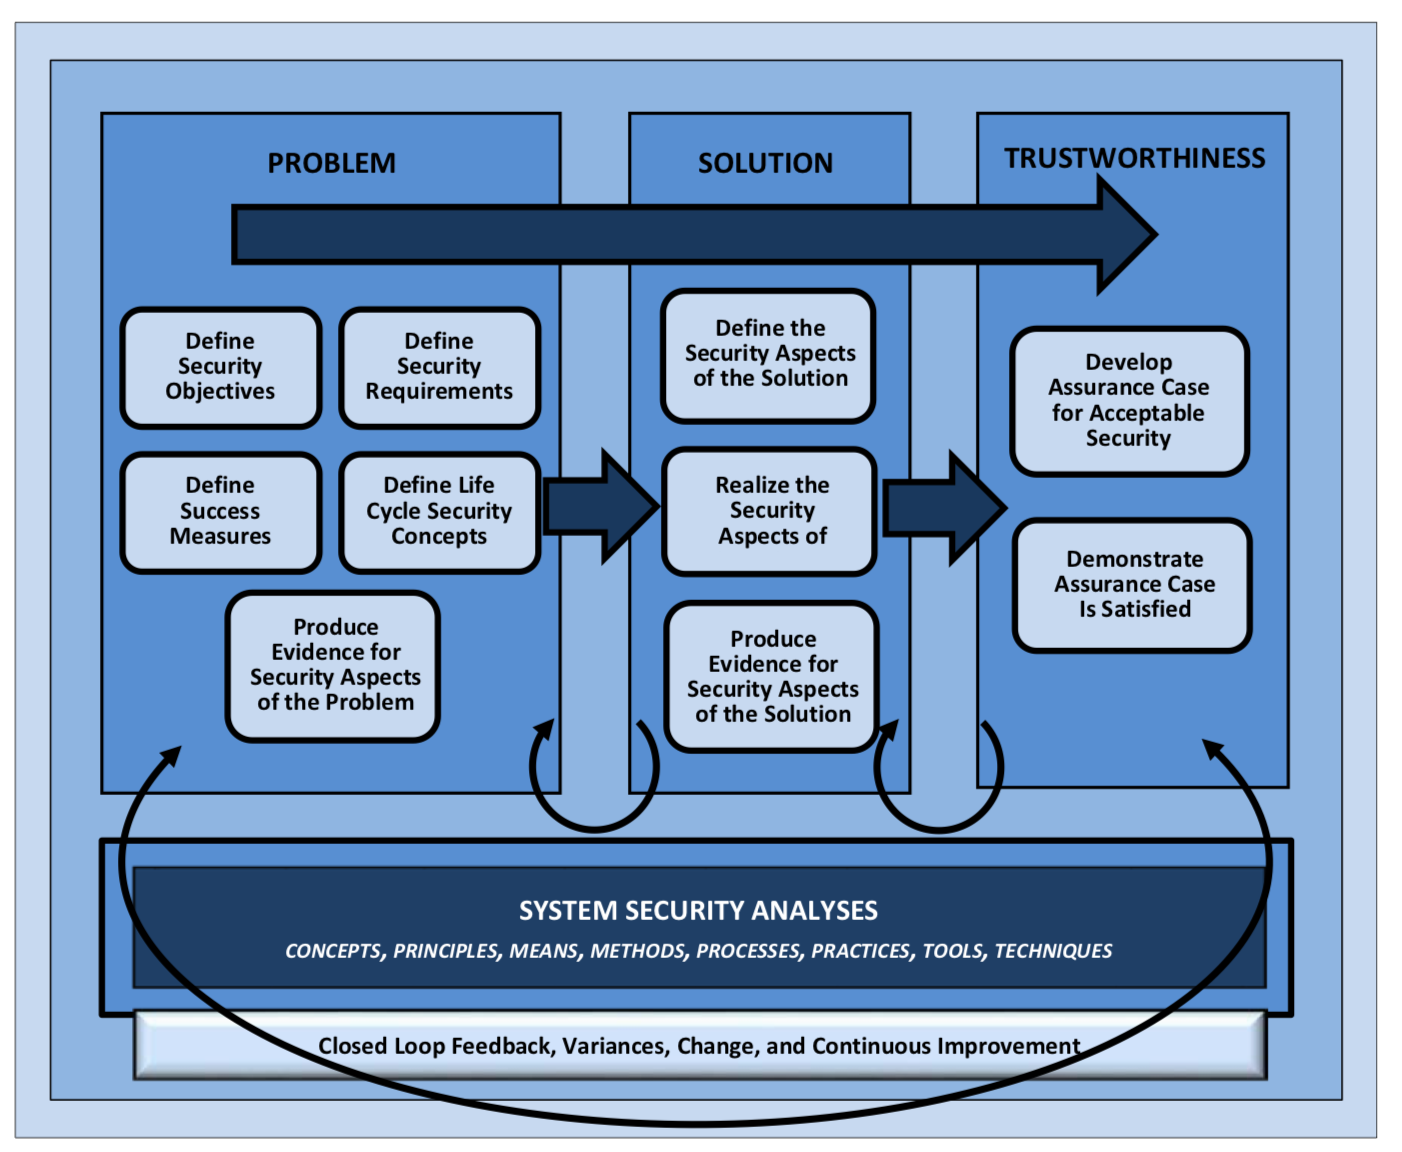
\includegraphics[width=\linewidth]{../figures/sseframework}
\caption{\label{sseframework}Systems security engineering Framework. (Image from \glsentryshort{nist} Special Publication 800-160 Vol 1: Systems Security Engineering Considerations for a Multidisciplinary Approach in the Engineering of Trustworthy Secure Systems.)}
\end{figure}

\paragraph*{Problem}
The framework describes the problem, solution, and trustworthiness activity contexts.  These three contexts are further broken down.  The problem phase focuses on defining security from the stakeholder's needs, purpose, and mission.  It is divided into four subcategories.  The first category defines the security objective. What does it means to be "\textit{adequately secure}"?   What are the assets and asset losses?  Which losses are unacceptable?
 
The second category in the problem context is to define measures of success.  What level of asset protection is required?  What level of assurance or protection is required?  

The third subcategory is to define the system life-cycle security concepts.  What is the system security context throughout the life-cycle of the system?  What processes, methods, and procedures throughout the system's life cycle need security?  

The fourth subcategory is to define the security requirements.  The stakeholder security requirements are determined from the previous three subcategories.

\paragraph*{Solution}
With the problem defined, the solution activity transforms the problem into security design requirements.  This a three part process.  The first subcategory in the solution context is to define the security aspects of the solution. NIST SP 800-160 lists six aspects to focus on: protection strategy; security design requirements; security architecture view and viewpoints; security design; security procedural aspects, capabilities, and limitations in the system life-cycle; and how to verify and measure security performance. 

The next subcategory is to realize the security aspects.  This is the security implementation phase.

The last subcategory in the solution context is to produce evidence for the security aspects of the solution. This assurance evidence can be obtained from a variety of SSE verification methods.  Assurance claims are measured against the stakeholder's requirements.

\paragraph*{Trustworthiness}
Once the solution is generated, the trustworthiness context provides evidence that the system is trustworthy.  The evidence supports the security objective claims.  There are two subcategories of activities in this context.  The first is to develop and maintain that assurance case for acceptable security.  NIST SP 800-160 defines assurance case as \textit{"a well-defined and structured set of arguments and a body of evidence showing that a system satisfies specific claims with respect to a given quality attribute."}  Assurance cases also provide auditable artifacts supporting the system security claims.

The other trustworthiness activity is to demonstrate that the assurance case is satisfied.  As subject-matter expert should evaluate the assurance case to determine if the evidence supports the security claims.

\subsubsection{Conforming to The SSE Framework}
The STORM methodology is intended to conform to the SSE Framework.  It is up to the STORM user to verify in detail that \textit{all} nine sub-contexts of the SSE Framework are addressed.  Proper application of STORM and system engineering thinking is sufficient for this.

STORM is composed of two components (described next), STPA and CSBD.  STPA focuses on the problem and solution contexts of the framework.  The problem is defined by the STPA analysis.  The solutions should evolve from implementing the constraints derived from this analyisis. CSBD focuses on demonstrating trustworthiness through formal methods and computer-aided reasoning.  It uses a rigorous mathematical logic to verify claims of security with regards to confidentiality, integrity, and accessibility.  It produces an auditable and reproducible document that should be included with the system documentation.

The work in this master thesis applies the STORM methodology to patrol base operations. 


%%%%%%%%%%%%%%%%%%%%% Section STORM %%%%%%%%%%%%%%%
\section{STORM}\label{sec:storm}

STORM is an approach to engineering trustworthy systems that satisfy stakeholder and conform to the SSE framework.  It applies state-of-the-field analysis techniques to design products that are safe, secure, and integral.  It applies formal methods to produce reproducible and auditable verification demonstrating that stakeholder claims are satisfied.


STORM is a new approach to implementing the Systems Security Framework.  It the result of the collaborative effort of Professor Shiu-Kai Chin of the College of Engineering and Computer Science at Syracuse University, Erich Devendorf, PhD of the U.S. Air Force Research Laboratory, and William Young, PhD of the U.S. Air Force 53rd Electronic Warfare Group.  STPA-Sec is the work of Dr. Young, who presented it as his PhD thesis in 2014 at MIT.  CSBD is derived from the work of Professor Shiu-kai Chin and Professor Susan Older (also of the College of Engineering and Computer Science at Syracuse University).  They wrote the text on \textit{Access Control, Security, and Trust: A Logical Approach} \cite{csbd} from which CSBD is derived.  Professor Shiu-Kai Chin teaches components of CSBD at Syracuse University in the College of Engineering and Computer Science.  


All elements of STORM are currently employed by the U.S. Air Force.  Components of STORM are taught at Syracuse University, in particular CSBD.  STPA-Sec is part of the U.S. Air Force doctrine.  CSBD has been used in the design of JP Morgan Company's SWIFT protocols \cite{} and the F-16 Viper payload controller and secure memory loader verifier (not published). As this master thesis is being written, STORM is being presented to the National Security Agency (NSA) for inclusion into their ? program.


%%%%%%%%%%%%%%%%%%%%% Subsection STORM %%%%%%%%%%%%%%%
\subsection{STAMP}\label{ssec:stamp}
System-Theoretic Accident Model and Processes (STAMP) underlies the STPA approach.  Figure \ref{stampstpa} shows the relationship between STPA-Sec, STPA, and STAMP.


STAMP is a way of thinking about how accidents occur.  It assumes both a traditional and a system-theoretic view.  In the traditional view, accidents are caused by unsafe chains of events.  In the system theoretic view, accidents are also caused by dynamic and complex interactions. System theory focuses on the system as a whole rather than as a collection of subcomponents.  The need for a system theory approach is epitomized in the notion that the whole is greater than the sum of its parts.  From the complex interactions of individual components arise emergent properties. These properties can be thought of as a higher order that is not predictable from the behavior of the individual components.





\begin{figure}[h!]
\centering
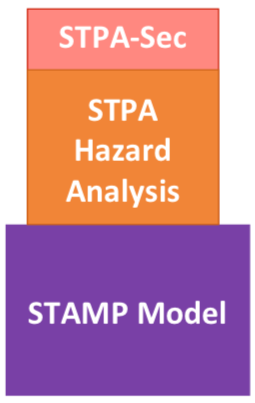
\includegraphics[width=0.3\linewidth]{../figures/stampstpa}
\caption{\label{stampstpa}Relationship between STPA-Sec, STPA, and STAMP.  Image from Dr. William Young and Reed Prada 2017 STAMP Conference presentation in Boston, MA on March 27, 2017 \cite{youngPorada} }
\end{figure}

STAMP had its inception in the mind of Massachusetts Institute of Technology Professor Nancy Leveson near the turn of the twenty-first century. It grew out of a frustration with the state-of-the-art in safety analysis tools.  These tools, at one time effective, were proving ineffective on the complexities associated with technologies of the modern era.  Modern technologies exhibited emergent properties arising from complex interactions among multiple components.  The practice of analyzing individual component reliability and chain-of-causality failures did not capture the hazards associated with these more complex systems.  A new systems-theoretic way of thinking was needed.  

STAMP forms the foundation of modern era safety analysis techniques.  Several approaches to safety engineering are built upon the STAMP foundation.  System-Theoretic Process Analysis (STPA) is one these analysis techniques.  In addition to STPA (the topic of the next section), several other analysis techniques are built on top of the STAMP foundation.  These include Causal Analysis based on Systems Theory (CAST), STPA for security (STPA-Sec), STPA for privacy (STPA-Pric), STPA-SafeSec \cite{safe}, and SAFE (a refinement focused on hardware and software subsystems \cite{safe}.

STAMP is a relatively new model that is rapidly growing in popularity.  It is the subject of yearly conferences world wide promoted by the Partnership for Systems Approaches to Safety and Security (PSASS)\footnote{See \url{https://psas.scripts.mit.edu/home/other-stamp-meetings/}.}.  When compared to other accident models, STAMP is more effective \footnote{See, for example, Paul Stukus' thesis dissertation on how STAMP outdid other techniques when analyzing a U.S. Coast Guard Buoy Tender Integrated Control System \cite{buoy}}.  It also cost less to implement \cite{stpa}.


STAMP takes a top-down view of accidents as dynamic control problems that arise out of complexity.  It focuses on safety constraints, hierarchical control structures, and process models \cite{saferworld}. 

\paragraph*{safety constraints}
STAMP views constraints, rather than events, as the safety-critical processes.  A lack of constraints can lead to a hazardous system state which will lead to an accident in the worst-case scenario.  

There are two types of constraints (or controls), passive and active.  Passive controls prevent unsafe conditions by their presence.  For example, lead shielding surrounding radioactive material minimizes radioactive exposure merely by its presence.  

Active controls, on the other hand, are more complicated.  They require some form of interaction to prevent unsafe conditions.  For example, a Geiger counter signaling a computer that radioactive levels are unsafe minimizes exposure by sounding an alarm which causes personnel to evacuate.  

\paragraph*{hierarchical control structures}
Figure \ref{controlmodel} is an example of a hierarchical control model.  The level of control funs from top to bottom.  Downward pointing arrows indicate instructions to lower level controllers or controlled processes.  Upward pointing arrows indicate feedback from lower components.   

\begin{figure}[h!]
\centering
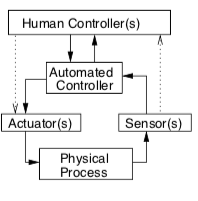
\includegraphics[width=0.5\linewidth]{../figures/controlmodel}
\caption{\label{controlmodel} Example of a control model. (Image captured from the \glsentryshort{stpa} Handbook \cite{stpa}.)}
\end{figure}
Higher-level control structures control lower-level control structures.  Inadequate control at higher levels trickle down to lower levels causing hazardous conditions.  STAMP considers four types of inadequate control on constraints: insufficient or missing constraints, wrong constraints, out-of-order or under-timed constraints, and constraints that are imposed for too long. 

\paragraph*{process models}
Figure \ref{processmodel} shows a controller with a process model.  Each controller has its own process model.  The process model describes the controller's model of the system.  If the controller's process model is not consistent with systems state, then unsafe control states may occur.

\begin{figure}[h!]
\centering
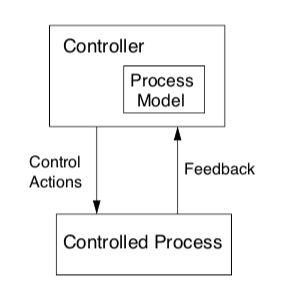
\includegraphics[width=0.5\linewidth]{../figures/processmodel}
\caption{\label{processmodel} Controller with process model. (Image captured from the \textit{Engineering a Safer World} Handbook \cite{safe}.)}
\end{figure}
%%%%%%%%%%%%%%%%%%%%% Subsection STORM %%%%%%%%%%%%%%%
\subsection{STPA/STPA-Sec}\label{ssec:stpa}
System-Theoretic Process Analysis (STPA) is a systems engineering methodology that helps the engineer identify and mitigate stakeholder losses. It does this using a four step process that is founded on the System-Theoretic Accident Model and Processes (STAMP).  Whereas STAMP is a way of thinking about the causes of accidents, STPA is a method to analyze systems in order to prevent or mitigate losses caused by these accidents.  

STPA follows the guidelines described in ISO/IEC/IEEE 15288 for System Life-Cycle Processes.  It's focus is on the Technical Processes (ISO/IEC/IEEE 15288), the concept and development stage of the system life cycle (defined in ISO/IEC/IEEE 24748), and the problem and solution contexts of the Systems Security Engineering Framework (NIST SP 800-160).


STPA, like STAMP, is the work of Professor Nancy Leveson from MIT.  STPA-Sec is William Young's (PhD and Col. in USAF) PhD thesis dissertation.  It is a modification of STPA that analyzes system security rather than just system safety.  In a 2013 paper, Professor Nancy Leveson and Dr. William Young define safety and security as
\begin{description}
\item[ Safety ] protecting a system against \textit{unintentional} disruptions.
\item[ Security ] protecting a system against \textit{intentional} disruptions.
\end{description}
The primary difference between STPA and STPA-Sec is that STPA thinks about how \textit{accidents} arise from system-level \textit{hazards} whereas STPA-Sec thinks about how \textit{losses} arise from system-level \textit{vulnerabilities}.  However, the application of the four STPA steps is the same.


\section{STPA/STPA-Sec Overview: Four Steps}
STPA is a four step process.  Figure \ref{4step} diagrams these four steps.  The four steps are briefly described below.  They are applied to the patrol base operations in the next chapter. 


\begin{figure}[h]
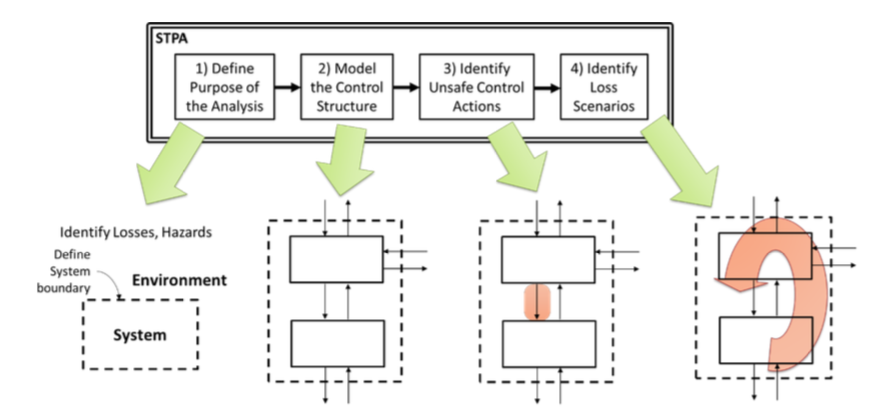
\includegraphics[width=\linewidth]{../figures/4step}
\caption{\label{4step} Four step process of STPA. (Image captured from the \textit{Engineering a Safer World} Handbook \cite{safe}.)}
\end{figure}

\paragraph*{Step 1: Define The Purpose of The Analysis}
The first step defines the purpose of the analysis, the system to be produced, and losses/accidents as defined by the stakeholders.  Vulnerabilities/hazards cause losses/accidents in worst-case scenarios.  In this step, losses/accidents are linked to vulnerabilities/hazards.  

System-level constraints are then defined and linked to vulnerabilities/hazards.  


\paragraph*{Step 2: Model The Control Structure}
The second step models the system.  The model is a functional control model that describes the flow in information in the system.  Figure \ref{controlmodel} shows an example of a control model.


\paragraph*{Step 3: Identify Unsafe Control Actions}
The next step identifies unsafe control actions (UCAs) for each control action described in step 2.  There are four types of UCAs.
\begin{itemize}
\item Not applying the control action
\item Applying the wrong control action
\item Applying the control action in the wrong order
\item Applying the control action for two long.
\end{itemize}


\paragraph*{Step 4: Identify Loss Scenarios}
The last step identifies scenarios that could cause the loss-linked control actions described in step 3.  This analysis should be used to guide system security engineering decisions.


%%%%%%%%%%%%%%%%%%%%% Subsection STORM %%%%%%%%%%%%%%%
\subsubsection{XSTAMPP}\label{sssec:xstamp}
XSTAMPP is an extensible application of STAMP that helps the user organize the STPA process.  XSTAMPP is built on the Eclipse IDE.  Eclipse allows users to write their own plug-ins for XSTAMPP.  Current plug-ins are STPA, STPA-Sec, STPA-Priv, STPA Verifier, and CAST.  


XSTAMPP was used for the STPA and STPA-Sec analysis.  However, at the time of this writing the program (and the data) were non-functional.
%%%%%%%%%%%%%%%%%%%%% Subsection STORM %%%%%%%%%%%%%%%
\subsection{CSBD}\label{ssec:csbd}
CSBD is a method for formally verifying and documenting the security properties of a systems.  It focuses on designing systems that satisfy the principle of complete mediation.  It uses an access-control logic (ACL) to reason about access to security sensitive objects.  It uses computer-aided reasoning such as the Higher Order Logic (HOL) Interactive theorem prover to formally verify and document these security properties.  The outcomes of CSBD applied to a system conform to the guidelines set fourth in System Security Engineering Framework, in particular by demonstrating that the assurance case is satisfied.

CSBD is described in more detail in chapter \ref{chp:csbdacl}.

%%%%%%%%%%%%%%%%%%%%% Subsection STORM %%%%%%%%%%%%%%%
\subsubsection{Confidentiality, Integrity, and Availability (CIA) }\label{sssect:ssmts}
At the core of security are the concepts of confidentiality, integrity, and availability.  Confidentiality refers to limiting access to objects (including information) by ensuring that only the right people (etc.\footnote{or any other "entity" that can request access to an object.}) have access to these things.  Confidentiality is the realm of things such as authentication and authorization.  Authentication means verifying a person's identity.  Authorization means describing a person's access rights. 

Integrity, on the other hand, refers to the whole of the object (or information, etc.).  It means controlling who or what can modify the object.   Integrity is the realm of things such as authorization.  In this case, authorization means describing a person's right to modify an object.  

Availability refers to accessibility.  Wikipedia describes availability as a measure of operability or degree to which the system is mission capable \cite {availability}. 

Confidentiality, integrity, and Availability are guarded by the principle of complete mediation.  


%%%%%%%%%%%%%%%%%%%%% Subsection STORM %%%%%%%%%%%%%%%
\subsubsection{Complete Mediation}\label{sssec:strommediate}
The seminal paper quoted on the principle of complete mediation is "The Protection of Information in Computer Systems" by Saltzer and Schroeder.  
\begin{quote}
\textit{
Complete mediation: Every access to every object must be checked for authority. This principle, when systematically applied, is the primary underpinning of the protection system. It forces a system-wide view of access control, which in addition to normal operation includes initialization, recovery, shutdown, and maintenance. It implies that a foolproof method of identifying the source of every request must be devised. It also requires that proposals to gain performance by remembering the result of an authority check be examined skeptically. If a change in authority occurs, such remembered results must be systematically updated.} \cite{saltzer}
\end{quote}

In summary, what this means is that any accessor attempting to access or modify a protected object must satisfy two conditions: (1) the accessor must be authenticated, and (2) the accessor must be authorized to access or modify that object.  This involves a three-step process: (1) defining the protected objects, (2) declaring who has what rights on these objects, and (3) defining how to verify the identity of the individual(s) accessing or modifying the objects.  

CSBD focuses on using an access-control logic and computer-aided reasoning to prove that a system satisfies the principle of complete mediation.

%%%%%%%%%%%%%%%%%%%%% Subsection STORM %%%%%%%%%%%%%%%
\subsubsection{Secure State Machines as Transition Systems }\label{sssect:ssmts}

Secure state machines are transition systems that enforce both constraints on the system and complete mediation.  They define allowable system states and allowable transitions among states. Transitions are overseen by a monitor which enforces complete mediation by only allowing transitions which are requested by an authenticated and authorized principal. 

Secure state machines are used by the CSBD method to enforce constraints on complete mediation.  (However, CSBD can also verify complete mediation without secure state machines.)
%%%%%%%%%%%%%%%%%%%%% Section PB %%%%%%%%%%%%%%%
\section{Patrol Base Operations}\label{sec:stormpb}
For the purpose of this master thesis, patrol base operations are an example of a non-automated, human-centered system wherein security is critical for mission success.  The operations are described in the U.S. Army Ranger Handbook.


Patrol base operations have a clear mission.  The activities are well-defined and mission-specific.  There is also a well-defined chain-of-command hierarchy.  Therefore, the patrol base operations are a great first example for testing the STORM methodology on a non-automated, human-centered system.  

But, the operations are also detailed and thus require some ingenuity in managing the level of detail.  This master thesis manages the detail by modeling the patrol base operations as a modularized hierarchy of secure state machines.  Each decreasing level of the hierarchy describes the operations in more detail (less abstraction).  As the level of detail increases, groups of details become modularized.  Patrol base operations are described in the next chapter and chapter \ref{chp:pb}.  
\end{document}